\documentclass[12pt,a4paper]{ctexart}

\usepackage[top=2.5cm,bottom=2.5cm,left=2cm,right=2cm]{geometry}
\usepackage{graphicx}
\usepackage[table]{xcolor}
\usepackage{booktabs}
\usepackage{float}
\usepackage{hyperref}
\usepackage{tabularx}
\usepackage{array}
\usepackage{caption}
\usepackage{enumitem}
\usepackage{zhnumber}

\definecolor{greenrate}{HTML}{C6EFCE}
\definecolor{yellowrate}{HTML}{FFEB9C}
\definecolor{redrate}{HTML}{FFC7CE}
\definecolor{headerbg}{HTML}{2F5496}
\definecolor{headerfg}{HTML}{FFFFFF}
\definecolor{grayrow}{HTML}{F2F2F2}
\definecolor{yellowrow}{HTML}{FFF2CC}
\definecolor{pinkrow}{HTML}{F4B4C2}

\graphicspath{{../figures/}{../分析结果/}}

\hypersetup{colorlinks=true,linkcolor=blue,urlcolor=blue}
\setenumerate[1]{itemsep=0pt,partopsep=0pt,parsep=0pt,topsep=0pt}
\setitemize[1]{itemsep=0pt,partopsep=0pt,parsep=0pt,topsep=0pt}
\setlength{\tabcolsep}{4pt}

\title{\textbf{408 计算机统考 — 全面分析报告}}
\author{数据管道: 习题册.xlsx → export\_xlsx\_to\_csv.py → analyze\_csv\_folder.py}
\date{\today}

\begin{document}
\maketitle
\thispagestyle{empty}
\newpage
\tableofcontents
\newpage

\section{四科总览}

\begin{table}[H]
\footnotesize
\centering
\begin{tabular}{lrrrrrr}
\hline
\rowcolor{headerbg}\textcolor{headerfg}{\textbf{科目}} & \textcolor{headerfg}{\textbf{题量}} & \textcolor{headerfg}{\textbf{正确数}} & \textcolor{headerfg}{\textbf{正确率}} & \textcolor{headerfg}{\textbf{已做章节}} & \textcolor{headerfg}{\textbf{已做小节}} & \textcolor{headerfg}{\textbf{状态}} \\
\textbf{数据结构} & 595 & 508 & \cellcolor{yellowrate}{85.4\%} & 8 & 28 & 一刷完成 \\
\textbf{计算机组成原理} & 592 & 437 & 73.8\% & 7 & 26 & 一刷完成 \\
\textbf{操作系统} & 650 & 484 & 74.5\% & 5 & 16 & 一刷完成 \\
\rowcolor{grayrow} 计算机网络 & — & — & 未开始 & — & — & 待开始 \\\\
\hline
\end{tabular}
\caption{四科完成总览}
\label{tab:overview}
\end{table}

\textbf{三科合计}：1429/1837 = \textbf{77.8\%}，408 估分约 \textbf{117 分}（满分 150）。
估分方式：章节正确率 $\times$ 150 直接折算。实际真题难度通常高于章节练习，得分可能略低 5—10 分。

\section{真题 vs 自编 章节对比}

\begin{figure}[H]
\centering
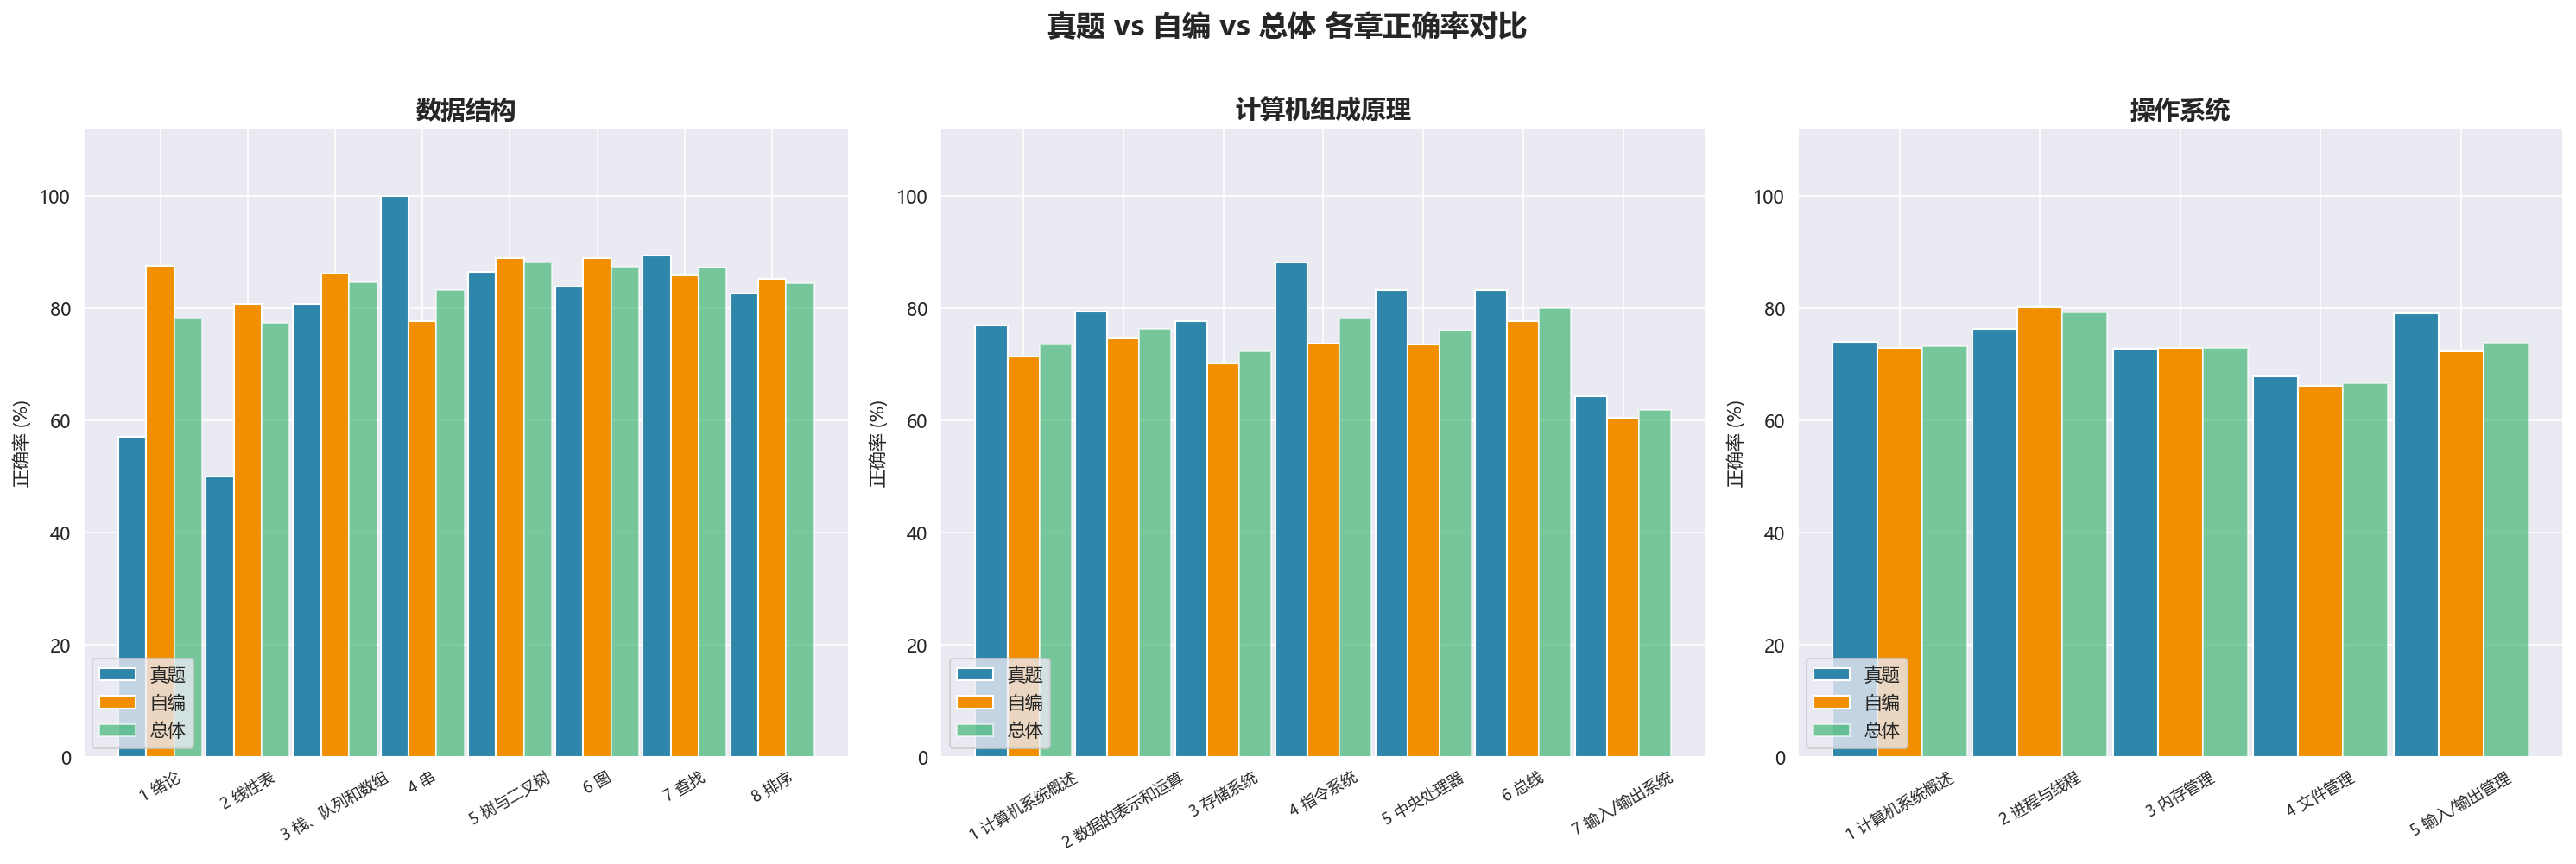
\includegraphics[width=0.92\textwidth]{408_zhenti_vs_zibian.png}
\caption{真题 vs 自编 vs 总体 各章正确率对比}
\end{figure}

\subsection{数据结构}

\begin{table}[H]
\footnotesize
\centering
\begin{tabular}{lrrrl}
\hline
\rowcolor{headerbg}\textcolor{headerfg}{\textbf{章节}} & \textcolor{headerfg}{\textbf{真题正确率}} & \textcolor{headerfg}{\textbf{自编正确率}} & \textcolor{headerfg}{\textbf{差距}} & \textcolor{headerfg}{\textbf{诊断}} \\
第 1 章  绪论 & \cellcolor{redrate}{57.1\%} & \cellcolor{yellowrate}{87.5\%} & -30pp & 自编优势 \\
第 2 章  线性表 & \cellcolor{redrate}{50.0\%} & \cellcolor{yellowrate}{80.9\%} & -31pp & 自编优势 \\
第 3 章  栈、队列和数组 & \cellcolor{yellowrate}{80.8\%} & \cellcolor{yellowrate}{86.2\%} & -5pp & 自编优势 \\
第 4 章  串 & \cellcolor{greenrate}{100.0\%} & 77.8\% & +22pp & 真题优势 \\
第 5 章  树与二叉树 & \cellcolor{yellowrate}{86.5\%} & \cellcolor{yellowrate}{88.9\%} & -2pp & 均衡 \\
第 6 章  图 & \cellcolor{yellowrate}{83.9\%} & \cellcolor{yellowrate}{88.9\%} & -5pp & 自编优势 \\
第 7 章  查找 & \cellcolor{yellowrate}{89.5\%} & \cellcolor{yellowrate}{85.9\%} & +4pp & 均衡 \\
第 8 章  排序 & \cellcolor{yellowrate}{82.6\%} & \cellcolor{yellowrate}{85.2\%} & -3pp & 均衡 \\
\hline
\end{tabular}
\caption{数据结构 真题 vs 自编}
\end{table}

\subsection{计算机组成原理}

\begin{table}[H]
\footnotesize
\centering
\begin{tabular}{lrrrl}
\hline
\rowcolor{headerbg}\textcolor{headerfg}{\textbf{章节}} & \textcolor{headerfg}{\textbf{真题正确率}} & \textcolor{headerfg}{\textbf{自编正确率}} & \textcolor{headerfg}{\textbf{差距}} & \textcolor{headerfg}{\textbf{诊断}} \\
第 1 章  计算机系统概述 & 76.9\% & 71.4\% & +5pp & 真题优势 \\
第 2 章  数据的表示和运算 & 79.5\% & 74.7\% & +5pp & 均衡 \\
第 3 章  存储系统 & 77.8\% & 70.2\% & +8pp & 真题优势 \\
第 4 章  指令系统 & \cellcolor{yellowrate}{88.2\%} & 73.7\% & +15pp & 真题优势 \\
第 5 章  中央处理器 & \cellcolor{yellowrate}{83.3\%} & 73.5\% & +10pp & 真题优势 \\
第 6 章  总线 & \cellcolor{yellowrate}{83.3\%} & 77.8\% & +6pp & 真题优势 \\
第 7 章  输入/输出系统 & \cellcolor{redrate}{64.3\%} & \cellcolor{redrate}{60.4\%} & +4pp & 均衡 \\
\hline
\end{tabular}
\caption{计算机组成原理 真题 vs 自编}
\end{table}

\subsection{操作系统}

\begin{table}[H]
\footnotesize
\centering
\begin{tabular}{lrrrl}
\hline
\rowcolor{headerbg}\textcolor{headerfg}{\textbf{章节}} & \textcolor{headerfg}{\textbf{真题正确率}} & \textcolor{headerfg}{\textbf{自编正确率}} & \textcolor{headerfg}{\textbf{差距}} & \textcolor{headerfg}{\textbf{诊断}} \\
第 1 章  计算机系统概述 & 74.1\% & 72.9\% & +1pp & 均衡 \\
第 2 章  进程与线程 & 76.3\% & \cellcolor{yellowrate}{80.2\%} & -4pp & 均衡 \\
第 3 章  内存管理 & 72.7\% & 73.0\% & -0pp & 均衡 \\
第 4 章  文件管理 & \cellcolor{redrate}{67.9\%} & \cellcolor{redrate}{66.2\%} & +2pp & 均衡 \\
第 5 章  输入/输出管理 & 79.2\% & 72.3\% & +7pp & 真题优势 \\
\hline
\end{tabular}
\caption{操作系统 真题 vs 自编}
\end{table}

\section{数据结构（85.4\%）}

题量：595 \quad 正确：508 \quad 章节：8 \quad 小节：28

\begin{figure}[H]
\centering

\includegraphics[width=0.92\textwidth]{04_王道数据结构/chapter_analysis.png}
\caption{章节与分布分析}
\end{figure}

\subsection{章节详情}

\begin{itemize}
\item \textbf{第 1 章  绪论} — 23 题，正确率 78.3\%。最弱：1.2 算法和算法评价（72.2%）
\item \textbf{第 2 章  线性表} — 53 题，正确率 77.4\%。最弱：2.3 线性表的链式表示（72.2%）
\item \textbf{第 3 章  栈、队列和数组} — 91 题，正确率 84.6\%。最弱：3.2 队列（75.0%）
\item \textbf{第 4 章  串} — 12 题，正确率 83.3\%。最弱：4.2 串的模式匹配（83.3%）
\item \textbf{第 5 章  树与二叉树} — 127 题，正确率 88.2\%。最弱：5.2 二叉树的概念（80.0%）
\item \textbf{第 6 章  图} — 103 题，正确率 87.4\%。最弱：6.3 图的遍历（77.8%）
\item \textbf{第 7 章  查找} — 102 题，正确率 87.3\%。最弱：7.3 树形查找（74.1%）
\item \textbf{第 8 章  排序} — 84 题，正确率 84.5\%。最弱：8.4 选择排序（76.2%）
\end{itemize}

\begin{figure}[H]
\centering

\includegraphics[width=0.92\textwidth]{04_王道数据结构/section_heatmap.png}
\caption{小节正确率热力图}
\end{figure}

\subsection{薄弱小节（< 70\%，共 0 个）}

\textbf{无} — 全部小节正确率 $\ge$ 70\%。

\subsection{掌握牢固（$\ge$ 90\%，共 12 个）}

1.1 数据结构的基本概念 (5/5)、2.1 线性表的定义和基本操作 (4/4)、8.1 排序的基本概念 (3/3)、7.5 散列(Hash)表 (23/24)、5.4 树、森林 (20/21)、6.2 图的存储及基本操作 (19/20)、6.1 图的基本概念 (17/18)、3.1 栈 (29/31)。

\section{计算机组成原理（73.8\%）}

题量：592 \quad 正确：437 \quad 章节：7 \quad 小节：26

\begin{figure}[H]
\centering

\includegraphics[width=0.92\textwidth]{03_王道计算机组成原理/chapter_analysis.png}
\caption{章节与分布分析}
\end{figure}

\subsection{章节详情}

\begin{itemize}
\item \textbf{第 1 章  计算机系统概述} — 34 题，正确率 73.5\%。最弱：1.3 计算机的性能指标（60.0%）
\item \textbf{第 2 章  数据的表示和运算} — 114 题，正确率 76.3\%。最弱：2.2 运算方法和运算电路（71.4%）
\item \textbf{第 3 章  存储系统} — 130 题，正确率 72.3\%。最弱：3.6 虚拟存储器（60.0%）
\item \textbf{第 4 章  指令系统} — 55 题，正确率 78.2\%。最弱：4.1 指令系统（75.0%）
\item \textbf{第 5 章  中央处理器} — 138 题，正确率 76.1\%。最弱：5.5 异常和中断机制（53.8%）
\item \textbf{第 6 章  总线} — 45 题，正确率 80.0\%。最弱：6.1 总线概述（80.0%）
\item \textbf{第 7 章  输入/输出系统} — 76 题，正确率 61.8\%。最弱：7.2 I/O接口（58.8%）
\end{itemize}

\begin{figure}[H]
\centering

\includegraphics[width=0.92\textwidth]{03_王道计算机组成原理/section_heatmap.png}
\caption{小节正确率热力图}
\end{figure}

\subsection{薄弱小节（< 70\%，共 8 个）}

\begin{table}[H]
\footnotesize
\centering
\begin{tabular}{lll}
\hline
\rowcolor{headerbg}\textcolor{headerfg}{\textbf{小节}} & \textcolor{headerfg}{\textbf{正确率}} & \textcolor{headerfg}{\textbf{建议}} \\
5.5 异常和中断机制 & \cellcolor{redrate}{53.8\%} (7/13) & \textbf{优先二刷} \\
7.2 I/O接口 & \cellcolor{redrate}{58.8\%} (10/17) & 重点回顾 \\
1.3 计算机的性能指标 & \cellcolor{redrate}{60.0\%} (12/20) & 重点回顾 \\
3.6 虚拟存储器 & \cellcolor{redrate}{60.0\%} (12/20) & 重点回顾 \\
7.3 I/O方式 & \cellcolor{redrate}{60.0\%} (33/55) & 重点回顾 \\
5.1 CPU的功能和基本结构 & \cellcolor{redrate}{62.5\%} (15/24) & 重点回顾 \\
3.5 高速缓冲存储器 & \cellcolor{redrate}{62.9\%} (22/35) & 重点回顾 \\
5.3 数据通路的功能和基本结构 & \cellcolor{redrate}{66.7\%} (12/18) & 查漏补缺 \\
\hline
\end{tabular}
\caption{计算机组成原理 薄弱小节}
\end{table}

\subsection{掌握牢固（$\ge$ 90\%，共 5 个）}

4.4 CISC和RISC的基本概念 (6/6)、7.1 I/O系统基本概念 (4/4)、5.6 指令流水线 (31/33)、1.2 计算机系统层次结构 (13/14)、3.1 存储器概述 (10/11)。

\section{操作系统（74.5\%）}

题量：650 \quad 正确：484 \quad 章节：5 \quad 小节：16

\begin{figure}[H]
\centering

\includegraphics[width=0.92\textwidth]{02_王道操作系统/chapter_analysis.png}
\caption{章节与分布分析}
\end{figure}

\subsection{章节详情}

\begin{itemize}
\item \textbf{第 1 章  计算机系统概述} — 86 题，正确率 73.3\%。最弱：1.6 虚拟机（63.6%）
\item \textbf{第 2 章  进程与线程} — 231 题，正确率 79.2\%。最弱：2.1 进程与线程简介（72.6%）
\item \textbf{第 3 章  内存管理} — 133 题，正确率 72.9\%。最弱：3.1 内存管理概念（70.8%）
\item \textbf{第 4 章  文件管理} — 93 题，正确率 66.7\%。最弱：4.2 目录与文件（60.0%）
\item \textbf{第 5 章  输入/输出管理} — 107 题，正确率 73.8\%。最弱：5.1 I/O管理概述（65.4%）
\end{itemize}

\begin{figure}[H]
\centering

\includegraphics[width=0.92\textwidth]{02_王道操作系统/section_heatmap.png}
\caption{小节正确率热力图}
\end{figure}

\subsection{薄弱小节（< 70\%，共 3 个）}

\begin{table}[H]
\footnotesize
\centering
\begin{tabular}{lll}
\hline
\rowcolor{headerbg}\textcolor{headerfg}{\textbf{小节}} & \textcolor{headerfg}{\textbf{正确率}} & \textcolor{headerfg}{\textbf{建议}} \\
4.2 目录与文件 & \cellcolor{redrate}{60.0\%} (42/70) & 重点回顾 \\
1.6 虚拟机 & \cellcolor{redrate}{63.6\%} (14/22) & 重点回顾 \\
5.1 I/O管理概述 & \cellcolor{redrate}{65.4\%} (17/26) & 查漏补缺 \\
\hline
\end{tabular}
\caption{操作系统 薄弱小节}
\end{table}

\subsection{掌握牢固（$\ge$ 90\%，共 2 个）}

4.1 文件系统基础 (5/5)、1.1 操作系统的基本概念 (10/11)。

\section{深度分析}

\subsection{错题绝对量 vs 正确率}

正确率相同时，错题量决定优先级。例如 CO I/O 方式错 22 题（55 题中），比中断错 6 题更需要时间投入。

\begin{figure}[H]
\centering
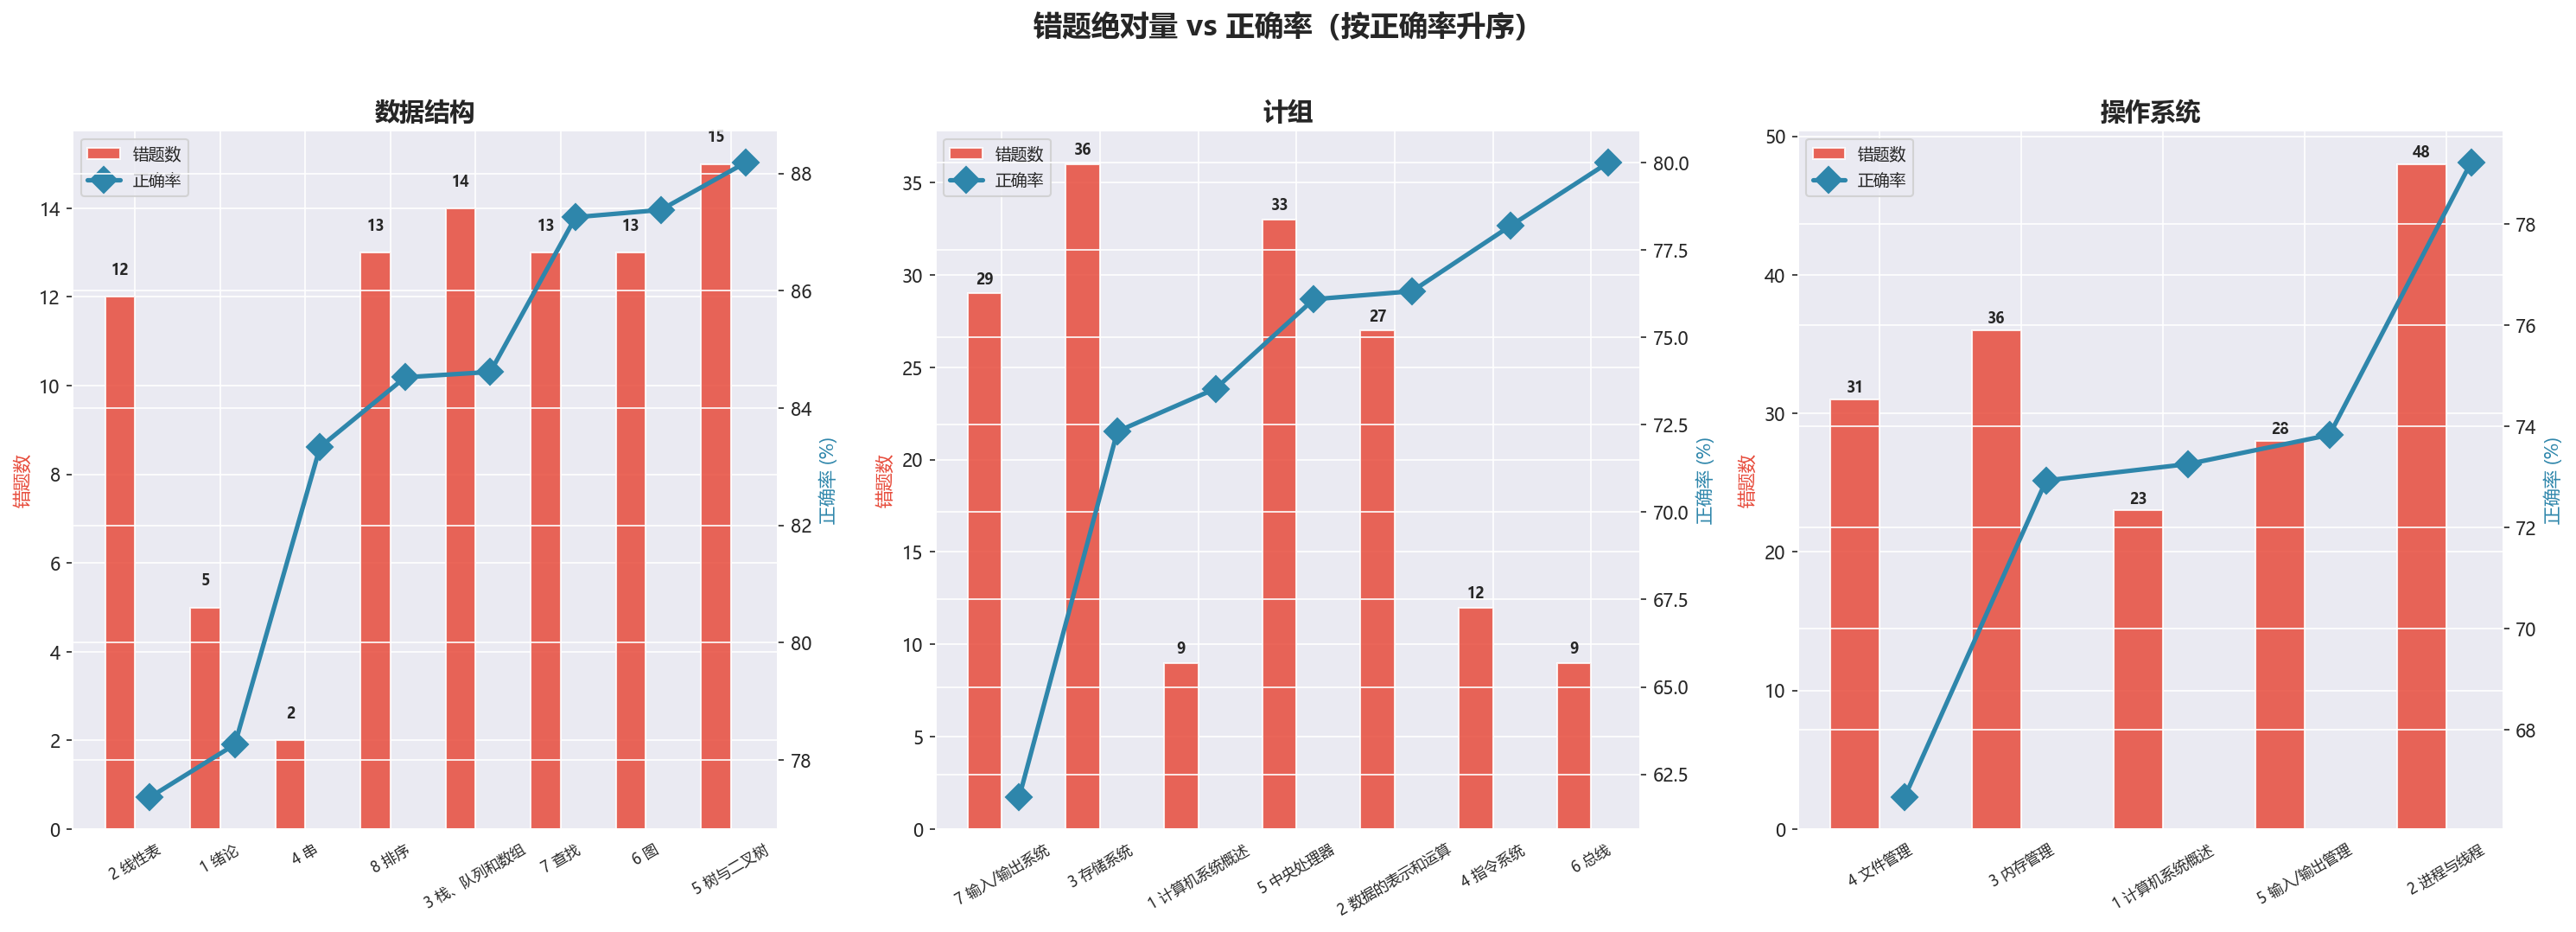
\includegraphics[width=0.92\textwidth]{408_wrong_count.png}
\caption{错题绝对量 vs 正确率}
\end{figure}

\subsection{题量-正确率象限图}

高题量+低正确率（气泡大且偏下）的章节是最大风险区。

\begin{figure}[H]
\centering
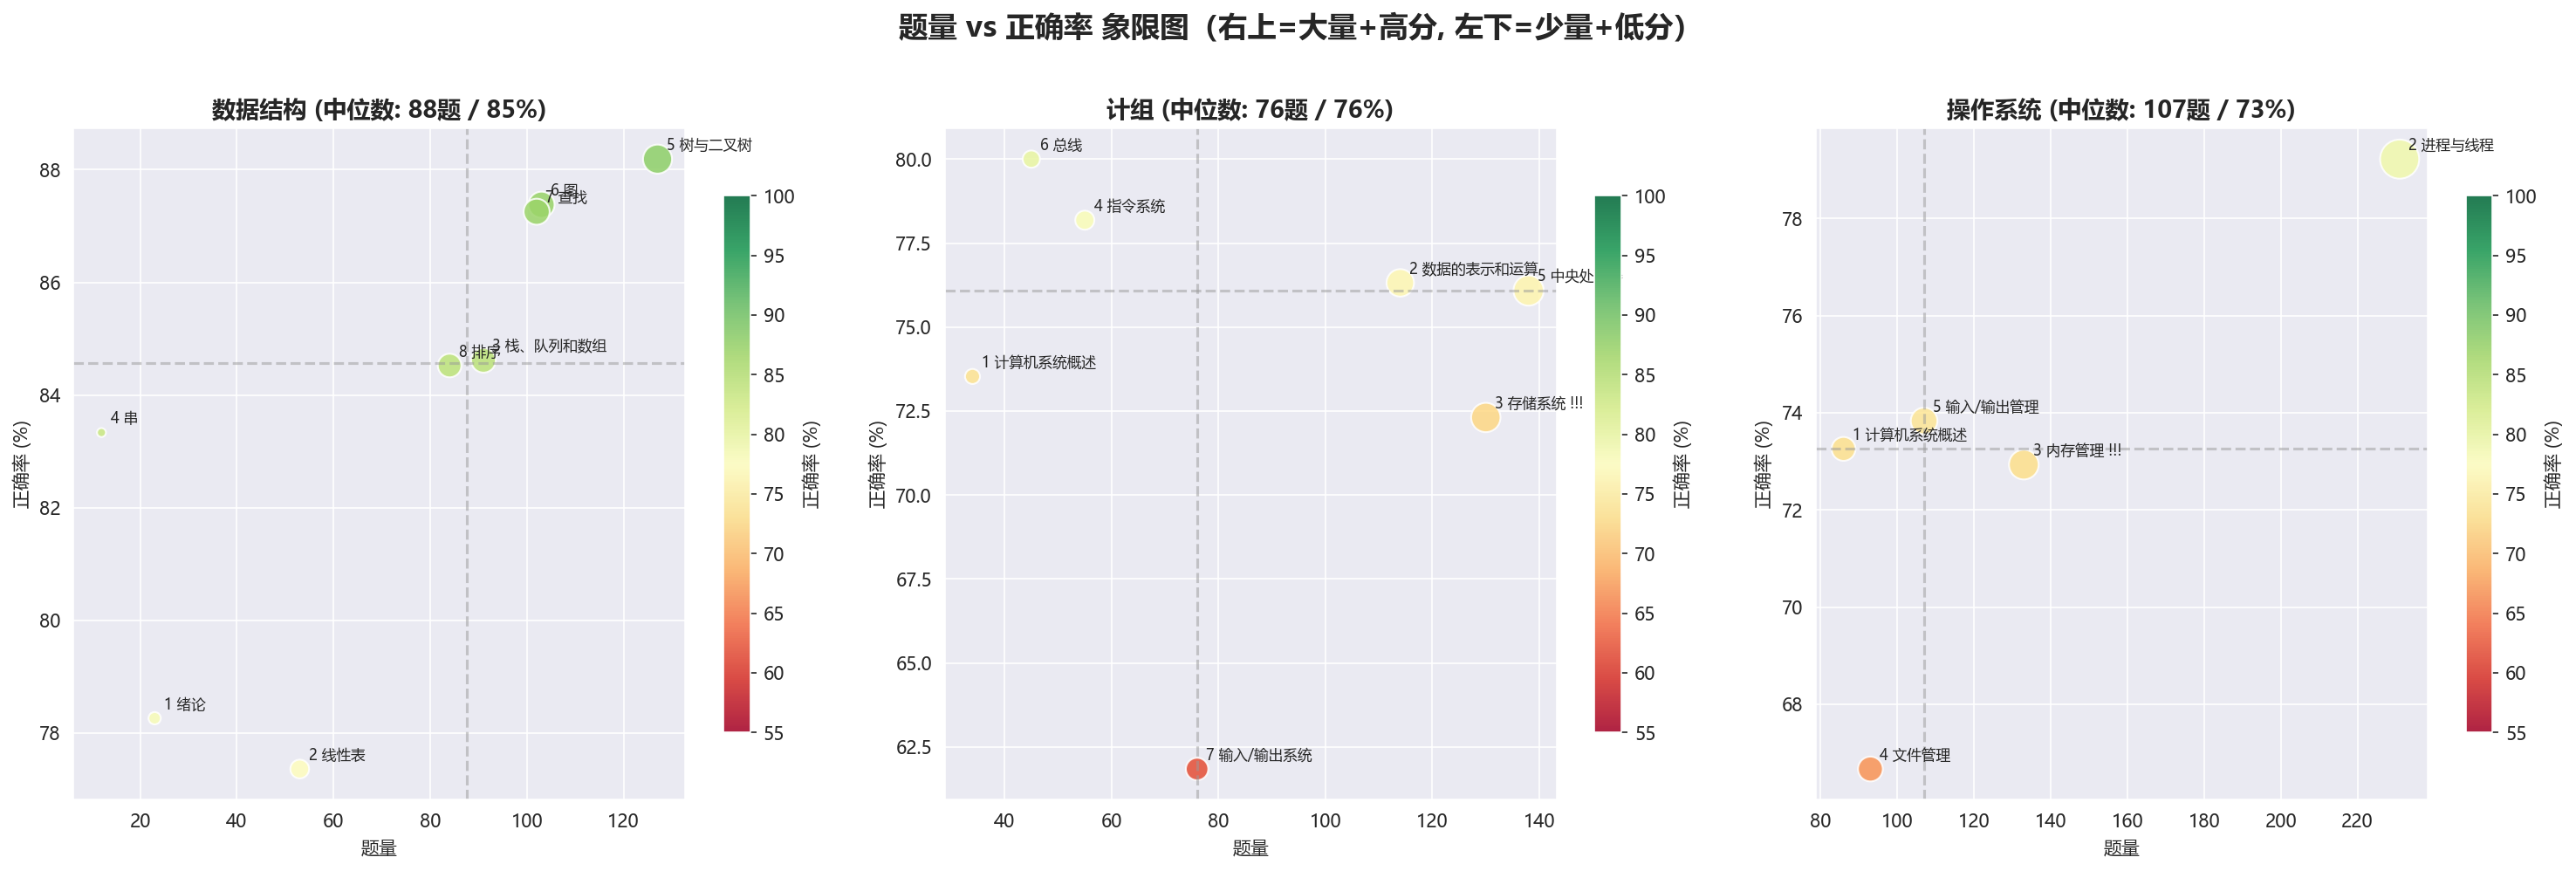
\includegraphics[width=0.92\textwidth]{408_quadrant.png}
\caption{题量-正确率象限图}
\end{figure}

\subsection{跨科关联：CO vs OS 重叠知识点}

408 命题常跨科综合。I/O 知识点 CO 62\% vs OS 74\%，差 12pp，问题在计组硬件层。

\begin{figure}[H]
\centering
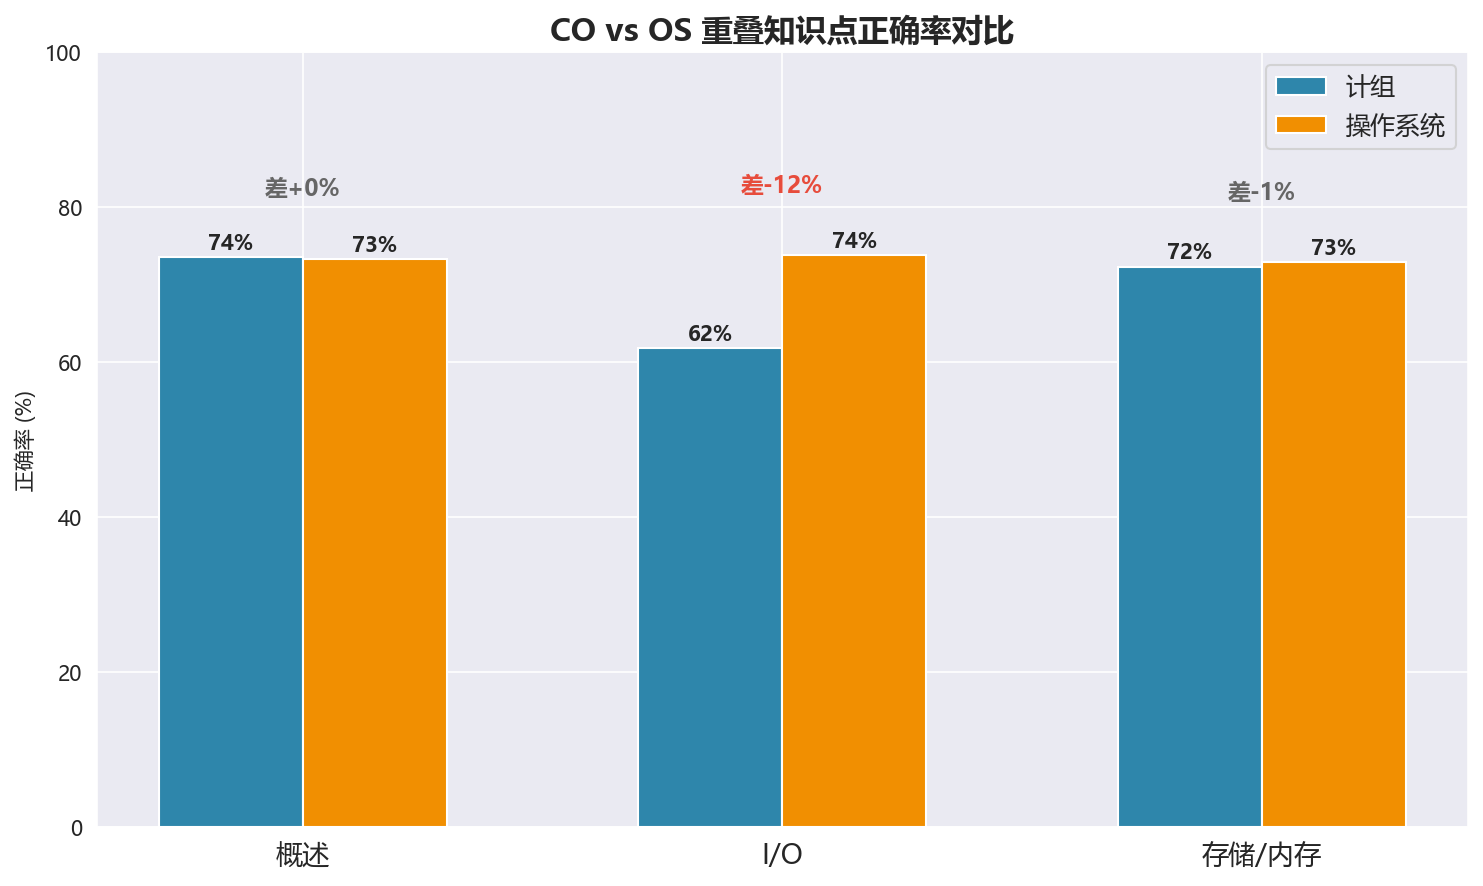
\includegraphics[width=0.92\textwidth]{408_cross_subject.png}
\caption{跨科关联：CO vs OS 重叠知识点}
\end{figure}

\subsection{目标差距量化（408 目标 125 分 → 每科 83\%）}

DS 85.4\% 已达标，CO 需 +9.2pp（约 54 题），OS 需 +8.5pp（约 55 题）。

\begin{figure}[H]
\centering
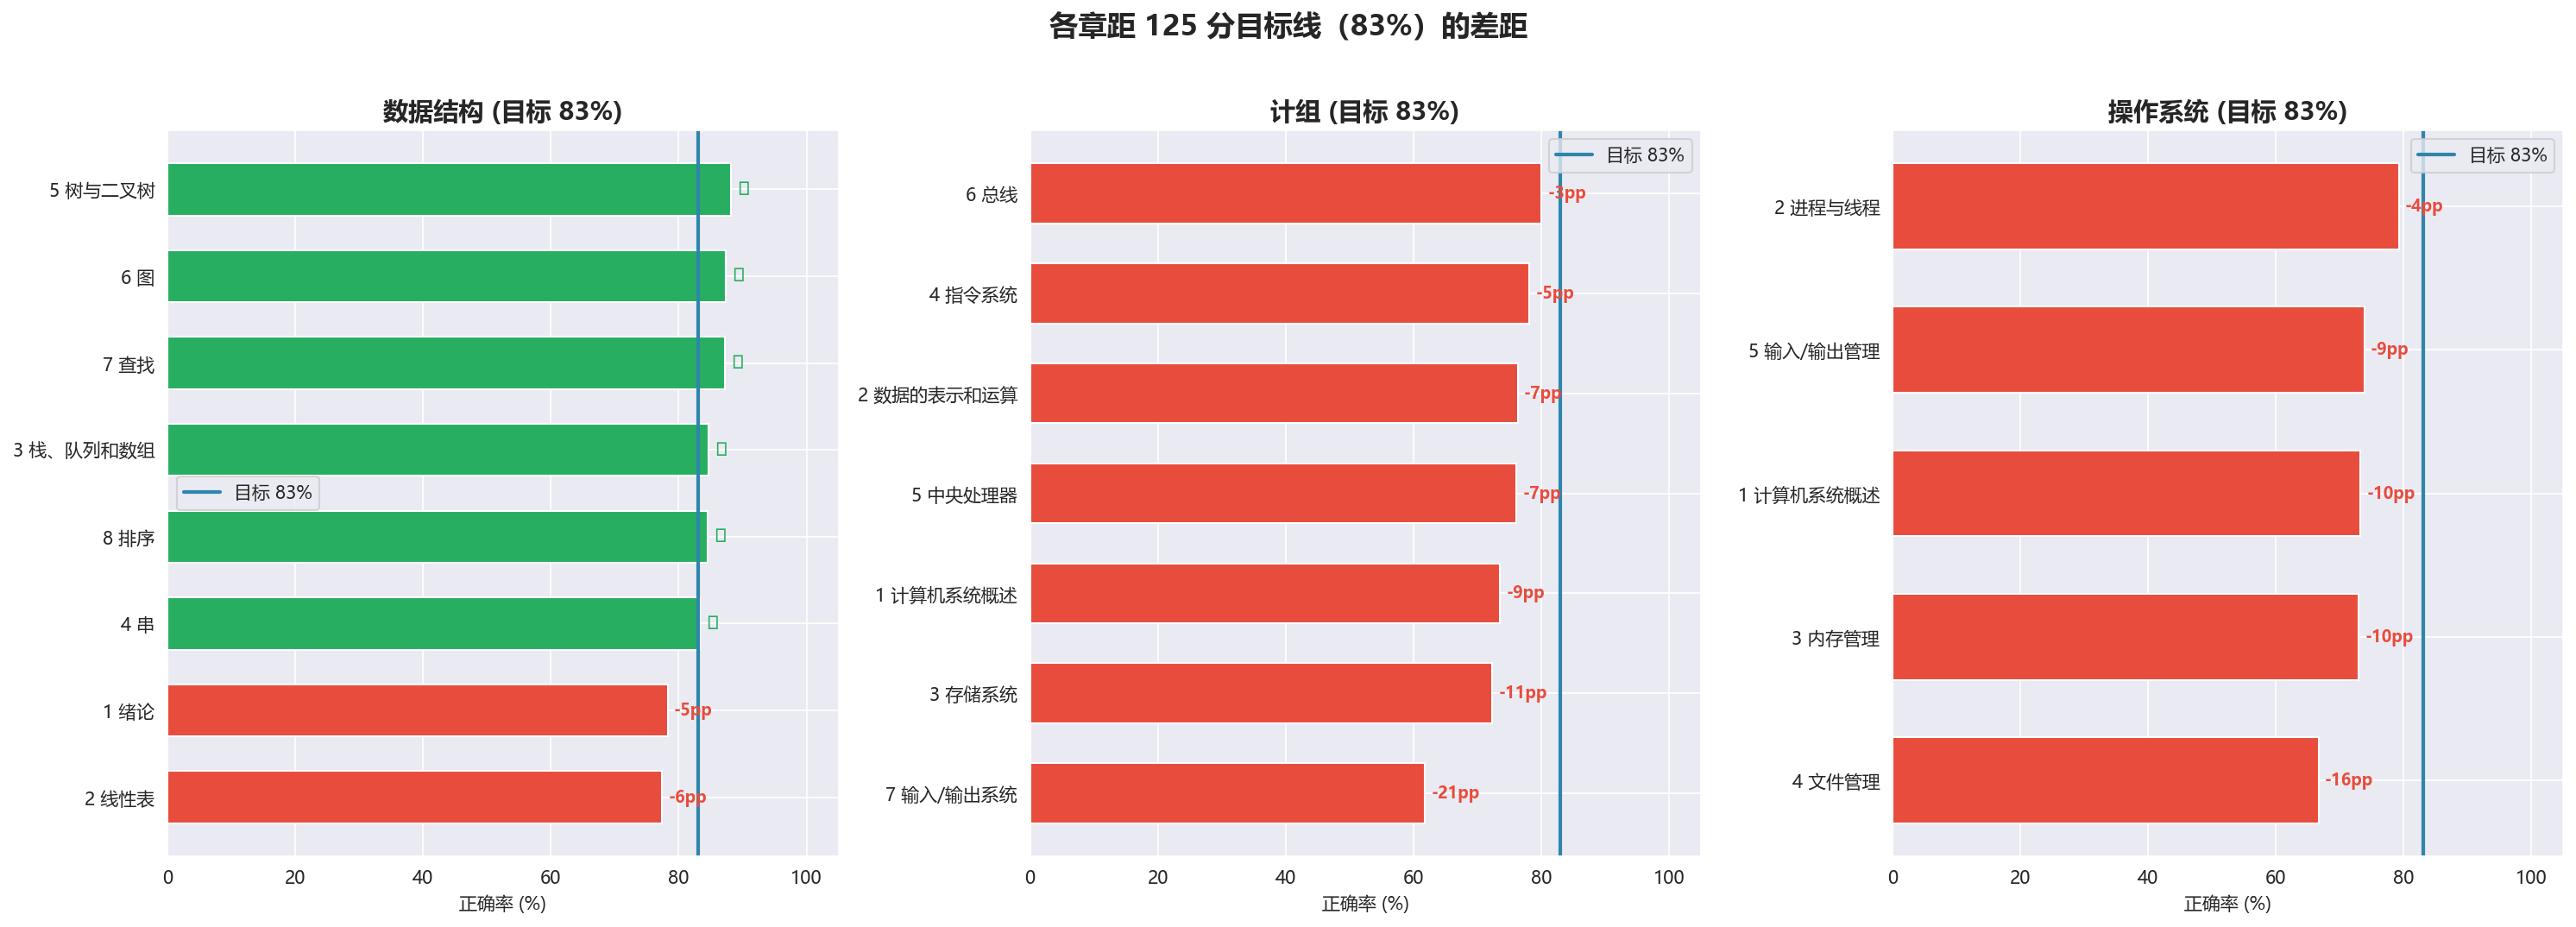
\includegraphics[width=0.92\textwidth]{408_target_gap.png}
\caption{目标差距量化（408 目标 125 分 → 每科 83\%）}
\end{figure}

\subsection{真题-自编差距显著性}

差距 $>$15pp 表示真题和自编考察角度差异大，需分别训练。DS 第1章(30pp)、第2章(31pp)自编远强于真题。

\begin{figure}[H]
\centering
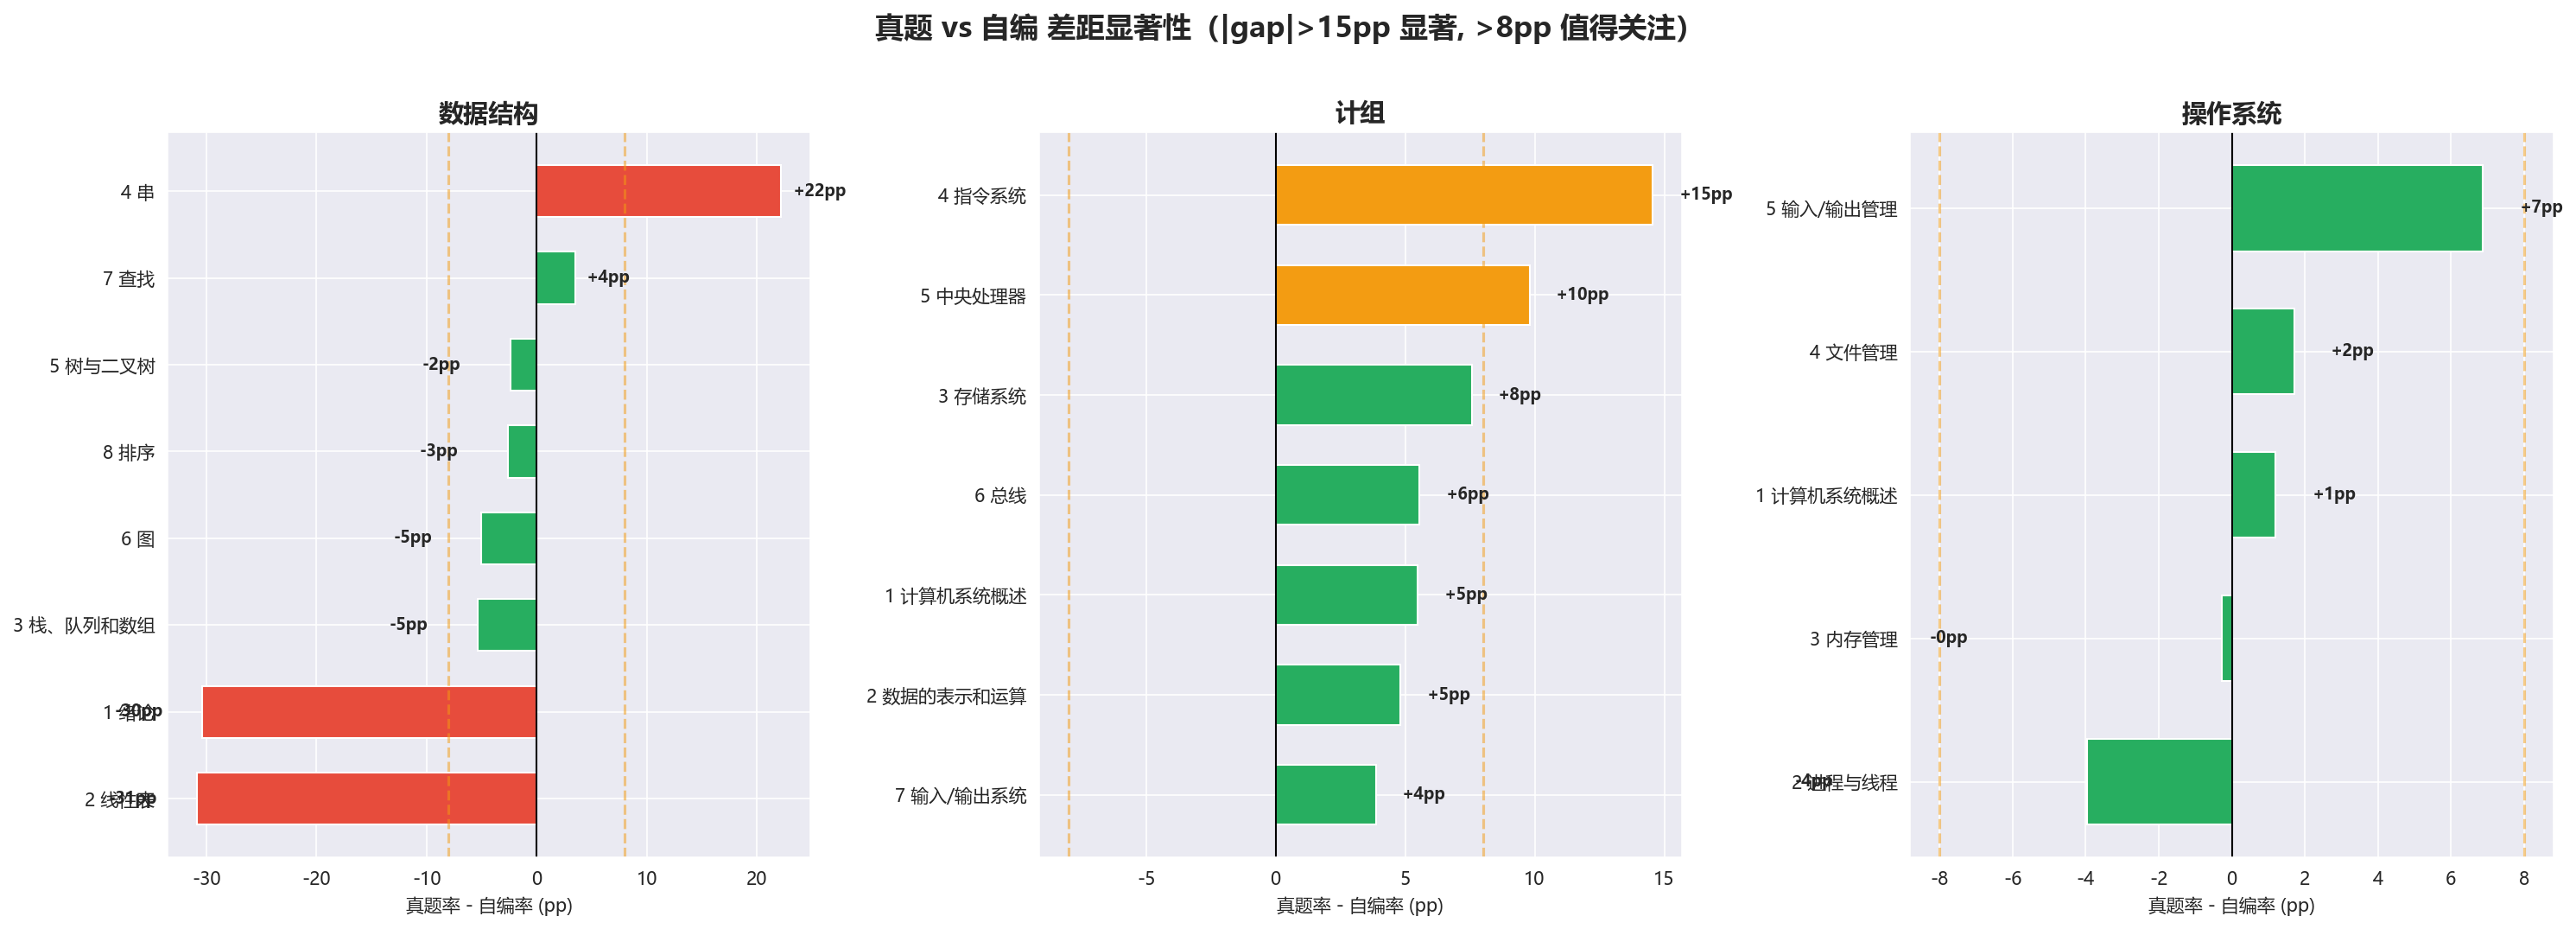
\includegraphics[width=0.92\textwidth]{408_gap_significance.png}
\caption{真题-自编差距显著性}
\end{figure}

\section{总结与建议}

\subsection{当前状态}

\begin{table}[H]
\footnotesize
\centering
\begin{tabular}{ll}
\hline
\rowcolor{headerbg}\textcolor{headerfg}{\textbf{指标}} & \textcolor{headerfg}{\textbf{数值}} \\
三科合计 & 1429/1837 = 77.8\% \\
408 估分 & 117 / 150 \\
已完成 & 3/4 科（DS/CO/OS） \\
DS 薄弱小节 & 0 个 \\
CO 薄弱小节 & 8 个 \\
OS 薄弱小节 & 3 个 \\
\hline
\end{tabular}
\caption{当前状态概览}
\end{table}

\subsection{优势}

\begin{itemize}
\item \textbf{DS 85.4\%}：树/图/查找/排序均 85\%+，0 个薄弱小节
\item CO 指令系统(78\%)和总线(80\%)达到良好水平
\item OS 进程管理(79\%)题量最大但正确率稳定
\end{itemize}

\subsection{短板与对策}

\begin{table}[H]
\footnotesize
\centering
\begin{tabular}{llll}
\hline
\rowcolor{headerbg}\textcolor{headerfg}{\textbf{短板}} & \textcolor{headerfg}{\textbf{当前}} & \textcolor{headerfg}{\textbf{目标}} & \textcolor{headerfg}{\textbf{对策}} \\
CO I/O 系统 & 61.8\% & 75\% & 中断+DMA+接口，3 小节全 < 70\% \\
CO 存储系统 & 72.3\% & 80\% & Cache+虚拟存储是 408 大题核心 \\
OS 文件管理 & 66.7\% & 78\% & 目录结构+文件分配，70 题 \\
计网 & 未开始 & 70\% & M 三步法：理解→分层→复盘 \\
\hline
\end{tabular}
\caption{短板与对策}
\end{table}

\subsection{下一步行动}

\begin{enumerate}
\item \textbf{计网开课} — 最后一块拼图，概念密集型
\item \textbf{CO I/O 二刷} — 仅 3 小节 76 题，2—3 天可完成
\item \textbf{OS 文件管理} — 70 题，与 I/O 穿插进行
\item \textbf{DS 维持} — 隔天 5—10 题保持手感
\end{enumerate}

\end{document}